\documentclass{article}
\usepackage{geometry}
 \geometry{
 a4paper,
 total={170mm,270mm},
 left=20mm,
 top=10mm,
 }
\usepackage{graphicx}
\usepackage{float}
\usepackage{enumitem}
\usepackage{caption}
\usepackage{amsmath}
\usepackage{datetime}
\usepackage{multirow}
\usepackage{listings}

\newcommand\blfootnote[1]{%
  \begingroup
  \renewcommand\thefootnote{}\footnote{#1}%
  \addtocounter{footnote}{-1}%
  \endgroup
}

\newdate{date}{20}{09}{2016}
\date{\displaydate{date}}
\title{\textbf{Network Analysis and Modelling - CSCI 5352} \\
Problem Set 2}
\author{\textbf{Santhanakrishnan Ramani}}
\begin{document}
\maketitle

\section*{Problem 1}
\begin{enumerate}[label=(\alph*)]
\item
Wkt, the mean degree of a random graph G(n,p) is $<k> = (n-1)p$. (From Lecture notes 3)\\
So for the group m, the expected degree for a vertex in G($n_m,p_m$) will be $<k> = (n_m-1)p_m$\\
Substituting the value of $p_m = A(n_m-1)^{-\beta}$ we get,$$<k> = (n_m-1)A(n_m-1)^{-\beta} = A(n_m-1)^{1-\beta}$$
 
\item
Wkt, the clustering coefficient of a random graph G(n,p) is $<C>=\dfrac{<k>}{(n-1)}$ (From Lecture notes 3)\\
So for the group m, the expected value $<C_m>$ of the local clustering coefficient for vertices in the group will be $<C_m> = <k>/(n_m-1)$. Substituting the value of $<k> = A(n_m-1)^{1-\beta}$ we get,
$$<C_m> = \dfrac{A(n_m-1)^{1-\beta}}{(n_m-1)} = A(n_m-1)^{-\beta}$$

\item
To show, $<C_m> \propto <k>^{{-\beta}/(1-\beta)}$\\
\underline{Proof:}
wkt,
$$<C_m> = \dfrac{<k>}{(n_m-1)}$$
Substituting $(n_m-1)$ in terms of $<k>$ by rearranging the equation in (a) we get,
$$<C_m> = \dfrac{<k>}{(\dfrac{<k>}{A})^{1/1-\beta}}$$
Since we interested only in $<k>$ throwing away the A from the equation above we get,
$$<C_m> \propto \dfrac{<k>}{<k>^{1/1-\beta}} = <k>^{1-1/1-\beta}$$
$$<C_m> \propto <k>^{-\beta/1-\beta}$$

To find the value of $\beta$ that has to assumed for the expected value of the local clustering coefficient to fall off as $<k>^{-0.75}$ as conjectured by some researchers, we equate the equation we got above to $<k>^{-0.75}$,

$$\dfrac{-\beta}{1-\beta} = -0.75$$
$$ \implies \beta = \dfrac{3}{7} $$
\end{enumerate}
\section*{Problem 2}
\begin{enumerate}[label=(\alph*)]
\item
Given a random graph G(n,p) with average degree c, we know that the number of triangles that can be formed in the given network is $\binom n3 p^3$. substituting, $p=c/(n-1)$ in it we get, (From Lecture notes 3)
$$no\_of\_triangles = \binom n3 (\frac{c}{(n-1)})^3 = \frac{n*(n-1)*(n-2)*c^3}{6*(n-1)^3} = \frac{n*(n-2)*c^3}{6*(n-1)^2}$$
Since here we are considering the limit of large n, we can approx $\dfrac{n*(n-2)}{(n-1)^2} = 1$, substituting in the equation above we get,
$no\_of\_triangles = \dfrac{1}{6}c^3$.\\

Since the formula is independent of n, the number of triangles is constant, neither growing nor vanishing in the limit of large n.

\item
Given a random graph G(n,p) with average degree c, we know that the number of connected triplets that can be formed in the given network is $\binom n3 p^2 * 3$. It is multiplied by 3 as there can be 3 different combinations of edge connections for the selected triple. Substituting, $p=c/(n-1)$ in it we get,

$$no\_of\_connected\_triples = \binom n3 (\frac{c}{(n-1)})^2 * 3 = \frac{n*(n-1)*(n-2)*c^2}{2*(n-1)^2} = \frac{n*(n-2)*c^2}{2*(n-1)} $$

Since here we are considering the limit of large n, we can approx $\dfrac{n*(n-2)}{(n-1)} = n$, substituting in the equation above we get, $no\_of\_connected\_triples = \dfrac{1}{2}nc^2$.

\item
According to Eq. (7.41) in Networks, 
\begin{center}
Clustering coefficient C = $\dfrac{\text{(number of triangles) * 3}}{\text{(number of connected triples)}}$
\end{center}
Substituting the values from (a) and (b) we get,
\begin{center}
Clustering coefficient C = $\dfrac{(\dfrac{1}{6})c^3*3}{(\dfrac{1}{2})nc^2} = \dfrac{c}{n}$
\end{center} 
We can clearly see that the value of Clustering coefficient C above agrees with Eq. (12.11) in Networks $C=\dfrac{c}{n-1}$ for large values of n, as n-1 can be approximated as n.
\end{enumerate}

\section*{Problem 3}
\blfootnote{Collaborated with Ruhi Saraf, Irene Beckman. Discussed the ideas and proofs for all the problems after trying on our own first.}
Given a undirected, unweighted network of n vertices that contains exactly two subnetworks of size $n_A$ and $n_B$, prove that the closeness centralities $C_A$ and $C_B$ of vertices A and B are related by 
$$\dfrac{1}{C_A} + \dfrac{n_A}{n} = \dfrac{1}{C_B} + \dfrac{n_B}{n}$$

\underline{Proof:}\\

wkt, the closeness centrality of vertex A is given by,
$$C_A = \dfrac{n}{\sum_{j=1}^{n} d_{Aj}} \implies
\dfrac{1}{C_A} = \dfrac{\sum_{j=1}^{n} d_{Aj}}{n}$$
\hspace{0.5 cm}
Now splitting,  $\sum_{j=1}^{n} d_{Aj} = \sum_{j=1}^{n_A} d_{Aj} + \sum_{j=1}^{n_B} d_{Aj} \;(as\; n = n_A + n_B)$ and substituting in the equation above\\

we get, $$\dfrac{1}{C_A} = \dfrac{\sum_{j=1}^{n_A} d_{Aj} + \sum_{j=1}^{n_B} d_{Aj}}{n}$$
\hspace{0.5 cm}
Since the distance of vertices in $n_B$ from A will be 1 plus distance from B (assuming all edges length = 1)
\begin{equation} \label{eq:1}
\dfrac{1}{C_A} = \dfrac{\sum_{j=1}^{n_A} d_{Aj} + \sum_{j=1}^{n_B} (1+d_{Bj})}{n}
= \dfrac{\sum_{j=1}^{n_A} d_{Aj} + \sum_{j=1}^{n_B} d_{Bj} + n_B}{n}
\end{equation}
\hspace{0.5 cm}
similarly,
\begin{equation} \label{eq:2}
\dfrac{1}{C_B} = \dfrac{\sum_{j=1}^{n_A} (1+d_{Aj}) + \sum_{j=1}^{n_B} d_{Bj}}{n} = \dfrac{\sum_{j=1}^{n_A} d_{Aj} + \sum_{j=1}^{n_B} d_{Bj} + n_A}{n}
\end{equation}
\hspace{0.5 cm}
from equations (\ref{eq:1}) and (\ref{eq:2}) above we get,
$$\dfrac{1}{C_A} - \dfrac{n_B}{n} = \dfrac{1}{C_B} - \dfrac{n_A}{n} \implies \dfrac{1}{C_A} + \dfrac{n_A}{n} = \dfrac{1}{C_B} + \dfrac{n_B}{n}$$

\section*{Problem 4}

Given an undirected (connected) tree of n vertices. Suppose that a particular
vertex in the tree has degree k, so that its removal would divide the tree into k disjoint regions, and suppose that the sizes of those regions are $n_1, . . . ,n_k$. Show that the betweenness centrality b of the vertex is $b = n^2 - \sum_{i=1}^{k} n^2_i$\\

wkt, betweenness centrality of a vertex $i$ is the total number of geodesic paths between all pairs of vertices $j$ \& $k$ in a given graph which passes through $i$. \\

Since the given tree is connected wkt every verted can be reached from any other vertes in the tree. There are $n$ vertices in the given tree, so the total numbers of pairs is $n^2$. \\

On removal of a vertex with degree $k$ we get k disjoint regions with size $n_1, . . . ,n_k$. So number of pairs in each disjoint set will be $n^2_i$ $(i=1,....,k)$. The sum of these pairs are the paths in the tree that doesn't pass through the vertex removed.\\

Therefore, the betweenness centrality of the vertex being removed is given by, $ b = n^2 - \sum_{i=1}^{k} n^2_i$

\section*{Problem 5}
\begin{itemize}
\item
The table \ref{table 1} and \ref{table 2} below lists the centrality scores for each vertex in the Medici family alliance network and lists within each centrality sorted in decreasing order of importance respectively.
\begin{table}[H]
\centering
\caption{Centrality Scores}
\label{table 1}
\begin{tabular}{|l|l|l|l|l|l|}
\hline
Node & Name         & Degree & Harmonic & Eigen & Betweenness \\
\hline
0    & Acciaiuoli   & 0.067  & 0.394    & 0.132 & 0.0         \\
1    & Albizzi      & 0.2    & 0.522    & 0.244 & 0.076       \\
2    & Barbadori    & 0.133  & 0.472    & 0.212 & 0.033       \\
3    & Bischeri     & 0.2    & 0.48     & 0.283 & 0.037       \\
4    & Castellani   & 0.2    & 0.461    & 0.259 & 0.02        \\
5    & Ginori       & 0.067  & 0.356    & 0.075 & 0.0         \\
6    & Guadagni     & 0.267  & 0.539    & 0.289 & 0.09        \\
7    & Lamberteschi & 0.067  & 0.358    & 0.089 & 0.0         \\
8    & Medici       & 0.4    & 0.633    & 0.43  & 0.186       \\
9    & Pazzi        & 0.067  & 0.318    & 0.045 & 0.0         \\
10   & Peruzzi      & 0.2    & 0.452    & 0.276 & 0.008       \\
11   & Pucci        & 0.0    & 0.0      & 0.0   & 0.0         \\
12   & Ridolfi      & 0.2    & 0.533    & 0.342 & 0.04        \\
13   & Salviati     & 0.133  & 0.439    & 0.146 & 0.051       \\
14   & Strozzi      & 0.267  & 0.522    & 0.356 & 0.036       \\
15   & Tornabuoni   & 0.2    & 0.522    & 0.326 & 0.033       \\
\hline    
\end{tabular}
\end{table}
\begin{table}[H]
\centering
\caption{Centrality Scores sorted in decreasing order of importance}
\label{table 2}
\begin{tabular}{|l|l|l|l|}
\hline
Degree                  & Harmonic                & Eigen                   & Betweenness           \\
\hline
('Medici', 0.4)         & ('Medici', 0.633)       & ('Medici', 0.43)        & ('Medici', 0.186)     \\
('Strozzi', 0.267)      & ('Guadagni', 0.539)     & ('Strozzi', 0.356)      & ('Guadagni', 0.09)    \\
('Guadagni', 0.267)     & ('Ridolfi', 0.533)      & ('Ridolfi', 0.342)      & ('Albizzi', 0.076)    \\
('Tornabuoni', 0.2)     & ('Tornabuoni', 0.522)   & ('Tornabuoni', 0.326)   & ('Salviati', 0.051)   \\
('Ridolfi', 0.2)        & ('Strozzi', 0.522)      & ('Guadagni', 0.289)     & ('Ridolfi', 0.04)     \\
('Peruzzi', 0.2)        & ('Albizzi', 0.522)      & ('Bischeri', 0.283)     & ('Bischeri', 0.037)   \\
('Castellani', 0.2)     & ('Bischeri', 0.48)      & ('Peruzzi', 0.276)      & ('Strozzi', 0.036)    \\
('Bischeri', 0.2)       & ('Barbadori', 0.472)    & ('Castellani', 0.259)   & ('Tornabuoni', 0.033) \\
('Albizzi', 0.2)        & ('Castellani', 0.461)   & ('Albizzi', 0.244)      & ('Barbadori', 0.033)  \\
('Salviati', 0.133)     & ('Peruzzi', 0.452)      & ('Barbadori', 0.212)    & ('Castellani', 0.02)  \\
('Barbadori', 0.133)    & ('Salviati', 0.439)     & ('Salviati', 0.146)     & ('Peruzzi', 0.008)    \\
('Pazzi', 0.067)        & ('Acciaiuoli', 0.394)   & ('Acciaiuoli', 0.132)   & ('Pucci', 0.0)        \\
('Lamberteschi', 0.067) & ('Lamberteschi', 0.358) & ('Lamberteschi', 0.089) & ('Pazzi', 0.0)        \\
('Ginori', 0.067)       & ('Ginori', 0.356)       & ('Ginori', 0.075)       & ('Lamberteschi', 0.0) \\
('Acciaiuoli', 0.067)   & ('Pazzi', 0.318)        & ('Pazzi', 0.045)        & ('Ginori', 0.0)       \\
('Pucci', 0.0)          & ('Pucci', 0.0)          & ('Pucci', 0.0)          & ('Acciaiuoli', 0.0)  \\
\hline
\end{tabular}
\end{table}

\begin{itemize}
\item
From table \ref{table 2} we can clearly see that the Medici family is at the top of the list of all the centrality measures calculated, which goes hand on hand with the Padgett and Ansell's explanation.

\item
\begin{itemize}
\item
From the scores, we can see that Guadagni family is second in the list of Harmonic, Degree and Betweenness centrality and Strozzi family is second in Degree and Eigen Vector Centrality score.
\item
The Degree Centrality of both the families are the same which can be attributed to the fact that both family possess the same number of degree.
\item
The Eigen Vector Centrality for the Strozzi is high compared to the Guadagni family which can attributed to the fact that the sum of degree of the nodes it is connected to is slightly more.
\item
The Harmonic Centrality of both the families are almost very close, the high score for the Guadagni family can be attributed to the fact it is very close to the Lamberteschi family which is at a larger distance from Strozzi family and all other families could be reached more or less at the same distance from both these families.
\item
The Betweenness Centrality of Guadagni family is high because of the reason it is the only way through which Lamberteschi family can be reached from all other families, whereas in case of Strozzi family the ones it is connected to can be reached without going through Strozzi family.
\end{itemize}
Therefore, either Guadagni or Strozzi family can be considered as the second most important family depending on what measures we consider.
\end{itemize}

\item

The figure below shows the difference between each vertex's harmonic centrality on the original network and its mean harmonic centrality under the configuration model with ${k_i}$ (degree sequence of the network), and also includes the 25 and 75\% quantiles around the mean.

\begin{figure}[!h]
  \centering
  \begin{minipage}[b]{0.5\textwidth}
    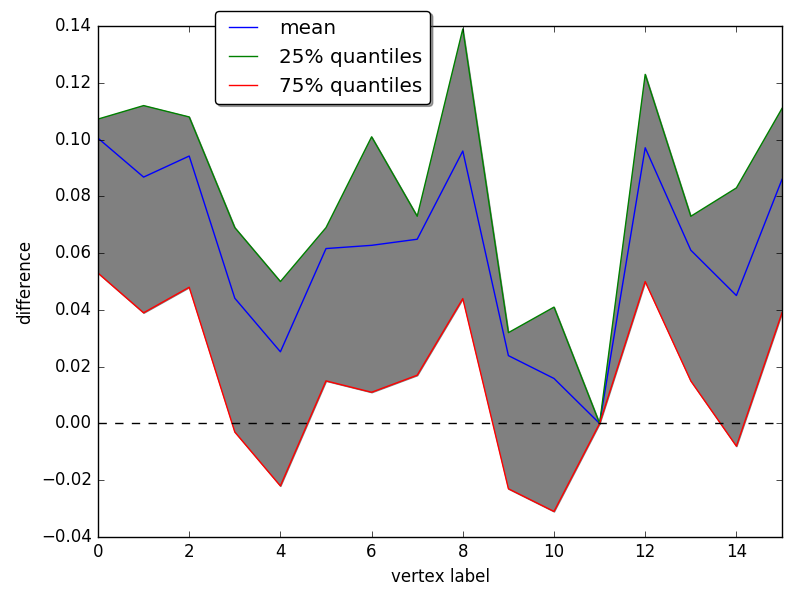
\includegraphics[width=\textwidth]{images/5b.png}
  \end{minipage}
\end{figure}

The figure above shows the difference between observed and expected centrality scores $\Delta$, where the line $\Delta = 0$ indicates no difference between observed and expected values. It is clear from the graph that the Observed value of centrality for the Medici's family is above this line indicating that they are more central than we would expect based on degree alone, and since the $\Delta = 0$ line lies outside the shaded region showing the 25 and 75\% quantiles on the distribution of centrality scores for each vertex, we can claim with some confidence that the observed value is different from the expected value. 

The behaviour observed completely agrees to Padgett and Ansell's story of the Medici family which states that the Medici's rising to power was focussed on establishing themselves as the most central players within the network of prominent Florentine families. 
\end{itemize}

\section*{Problem 6}
\begin{enumerate}[label=(\alph*)]
\item
The figure below represents the network in which distinct vertices hold the status of highest degree and betweenness centrality, and a table showing the ranking of the vertices and their centrality measures. \textbf{Vertex 2 \& 4} - High Degree Centrality and \textbf{Vertex 3} - High Betweenness Centrality.

\begin{center}
\begin{minipage}[b]{0.3\textwidth}
    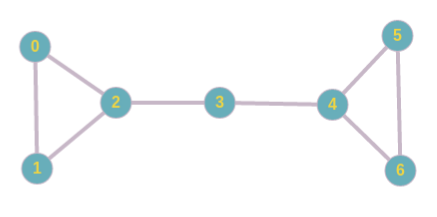
\includegraphics[width=\textwidth]{images/6a.png}
\end{minipage}
\begin{minipage}[b]{0.3\textwidth}
  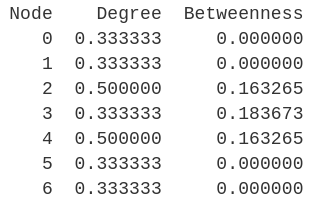
\includegraphics[width=\textwidth]{images/6a1.png}
\end{minipage} 
\end{center}
\end{enumerate}
\newpage
\section*{Code for Problem 5}
\begin{lstlisting}[language=Python]
def getEdges(G):
    edges = []
    name = []
    fileName = "/home/santa/Dropbox/NAM/Problem Set 2/Data/data_medici_network.txt"
    lines = [line.rstrip('\n') for line in open(fileName)]
    vertex=0
    for line in lines:
        G.add_node(vertex)
        openBracket = line.index('[')
        closeBracket = line.index(']')
        subStr = line[openBracket+1:closeBracket]
        list = []
        for i in range(len(subStr)):
            if subStr[i] == "(":
                word = ''
                while subStr[i+1] != ",":
                    i = i+1
                    word = word+subStr[i]
                list.append(word)
        for l in list:
            edges.append((vertex,int(l)))
        vertex=vertex+1
        name.append(line.split()[1].replace(",","").strip())
    return name, edges

def generateGraph():
    G = nx.Graph()
    name, edges = getEdges(G)
    G.add_edges_from(edges)
    return name, G 

def getDegreeCent(G):
    degreeCent = nx.degree_centrality(G)
    for k,v in degreeCent.items():
        degreeCent[k] = round(v,3)
    return degreeCent

def getHarmonicCent(G):
    harmonicCent = nx.harmonic_centrality(G)
    for k,v in harmonicCent.items():
        harmonicCent[k] = round(v/(G.number_of_nodes()-1),3)
    return harmonicCent

def getEigenCent(G):
    eigenCent = nx.eigenvector_centrality(G)
    for k,v in eigenCent.items():
        eigenCent[k] = round(v,3)
    return eigenCent

def getBetweenCent(G):
    betweenCent = nx.betweenness_centrality(G,normalized=False)
    for k,v in betweenCent.items():
        betweenCent[k] = round(v/(G.number_of_nodes()**2),3)
    return betweenCent
\end{lstlisting} 
\newpage 
\begin{lstlisting}[language=Python, breaklines=true] 
def calcCentralityScores():
    name, G = generateGraph
    data = {'Node' : pd.Series(range(G.number_of_nodes())),
            'Name' : pd.Series(name),
            'Degree' : pd.Series(getDegreeCent(G)),
            'Harmonic' : pd.Series(getHarmonicCent(G)),
            'Eigen' : pd.Series(getEigenCent(G)),
            'Betweenness' : pd.Series(getBetweenCent(G))}
    
    family = pd.DataFrame(data, columns=['Node', 'Name', 'Degree', 'Harmonic', 'Eigen', 'Betweenness'])
    #family.to_csv('/home/santa/Dropbox/NAM/Problem Set 2/Data/family.csv', index=False)
    
    data1 = {}
    for col in ['Degree', 'Harmonic', 'Eigen', 'Betweenness']:
        index = np.argsort(family[col])
        list = []
        for item in index[::-1]:
            list.append((name[item], round(family[col][item],3)))
        data1[col] = pd.Series(list)
    
    sort_family = pd.DataFrame(data1, columns=['Degree', 'Harmonic', 'Eigen', 'Betweenness'])
    #sort_family.to_csv('/home/santa/Dropbox/NAM/Problem Set 2/Data/sort_family.csv', index=False)

def getDegreeSeq():
    G = nx.Graph()
    name, edges = getEdges(G)
    G.add_edges_from(edges)
    return list(G.degree(G.nodes()).values())

def generateConfigModel():
    degreeSeq = getDegreeSeq()
    vector = []
    for i in range(len(degreeSeq)):
       for j in range(degreeSeq[i]):
           vector.append(i)
    
    noOfIter = 10000
    noOfNodes = len(degreeSeq)
    data = {}
    for i in range(noOfIter):
        random.shuffle(vector)
        edges = []
        for a,b in zip(vector[0:][::2],vector[1:][::2]):
            edges.append((a,b))
        G = nx.Graph()
        G.add_edges_from(edges)
        G.remove_edges_from(G.selfloop_edges())
        G.add_nodes_from(range(noOfNodes))
        data[i] = pd.Series(getHarmonicCent(G))
    
    configModel = pd.DataFrame(data)
    return configModel
\end{lstlisting}
\newpage 
\begin{lstlisting}[language=Python]   
def plotGraph():
    model_harmonic = generateConfigModel()
    name, G = generateGraph()
    orig_harmonic = pd.Series(getHarmonicCent(G))
    
    mean_diff = orig_harmonic - model_harmonic.mean(axis=1)
    quant_25  = orig_harmonic - model_harmonic.quantile(q=0.25,axis=1)
    quant_75  = orig_harmonic - model_harmonic.quantile(q=0.75,axis=1)
    
    plt.xlim(0,len(name)-1)
    plt.plot(mean_diff, label = 'mean')
    plt.plot(quant_25, label = '25% quantiles')
    plt.plot(quant_75, label = '75% quantiles')
    plt.plot(range(len(name)),[0]*len(name),'k--')
    plt.fill_between(range(len(name)),quant_25,quant_75, color='grey')
    plt.ylabel('difference')
    plt.xlabel('vertex label')
    plt.legend(loc='upper right', bbox_to_anchor=(0.5, 1.05), fancybox=True, shadow=True)
    plt.tight_layout()
    plt.show()
\end{lstlisting}
\end{document}
